\section{问题一　铭牌完整成像的可行区域}
设 \(d\in[0.30,1.50]\) 为相机到铭牌平面的垂直距离，\(u\in[-0.45,0.45]\) 为光轴相对铭牌中心的横向偏移。铭牌宽 0.24\,m，与图像传感器平面平行。采用针孔相机模型，忽略镜头畸变，并假定竖直方向有足够的取景余量。传感器横向有 960 个像素，令 \(t=\tan 30^\circ\)、\(w=0.24\)。距离 \(d\) 处的水平视野宽度为 \(2dt\)，故完整铭牌的投影像宽为 \(P(d)=960w/(2dt)\) 像素。设最低像宽为 \(P_0\)，铭牌左右两端均入镜且像宽达标的充要条件为
\begin{equation}
  d \leq \frac{960w}{2tP_0},\qquad
  |u|\leq \min(0.45,dt-w/2).
\end{equation}
若第二个不等式的右端为负，该距离下就没有可行的横向位置。将上述条件与夹具的机械行程取交集，得到图~\ref{fig:plate} 中的可行区域。将横向可用宽度 \(2\max(0,\min(0.45,dt-w/2))\) 沿可用距离积分，即得区域面积。当 \(P_0=200\) 时，\(d=0.987269\) 处开始允许使用全部横向行程；到 \(d=0.997661\) 处，像宽恰好降至下限。

\begin{figure}[H]\centering
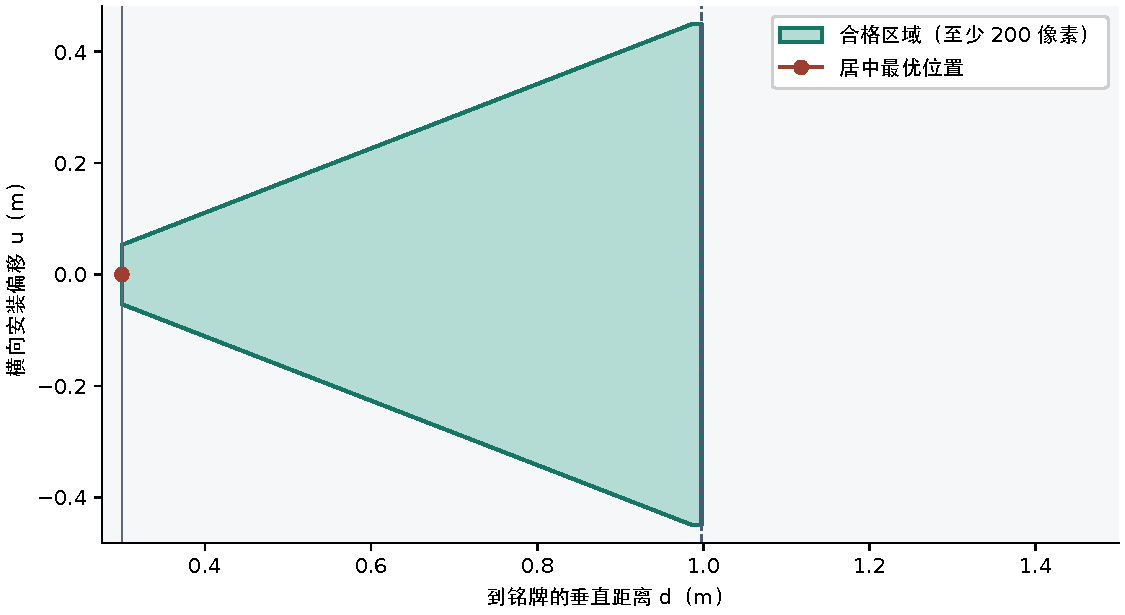
\includegraphics[width=.75\linewidth,height=.23\textheight,keepaspectratio]{label_region.pdf}
\caption{满足完整入镜和像宽要求的相机距离与横向偏移。}\label{fig:plate}
\end{figure}
\begin{table}[H]\centering
\caption{最低像宽对可行区域的影响。面积占比以夹具全部设置构成的 \(1.08\,\mathrm{m}^2\) 参数矩形为分母。}
\PlateTable
\end{table}
以投影像宽 \(P(d)\) 最大为目标。由于 \(P(d)\) 随 \(d\) 严格递减，当 \(d=0.30\) 时，凡满足 \(|u|\leq0.053205\) 的横向位置均为最优。取 \(u=0\) 居中放置，可以使左右两侧余量中较小的一侧也达到最大，两侧各余 147.45 像素。此时标称像宽为 665.11 像素。作为独立核验，在 \(9600\times6400\) 个网格单元的中点逐一投影铭牌的左右边缘；三个像宽门槛下，网格估计面积与积分结果的差均不超过 \(3.3\times10^{-5}\,\mathrm{m}^2\)。

\clearpage
\subsection{存在安装误差时的夹具设置}
理想条件下的最优解把相机设在允许的最近位置，安装时稍向铭牌靠近就会越过机械行程下限。设夹具的标称设置为 \((d_0,u_0)\)，实际位置可在 \(d_0\pm e,\ u_0\pm v\) 的范围内变化。这里的公差是算例设定，允许该矩形误差域内轴向和横向偏差的所有组合。

令 \(U=0.45\)、\(D=\min(1.50,960w/(2tP_0))\)。要使任何允许偏差下的实际位置均满足机械行程、左右边缘入镜和最低像宽要求，标称设置必须且只需满足
\begin{align}
 e+\max\{0.30,(w/2+v)/t\}\ \leq &\,d_0\leq D-e,\\
 |u_0|\ \leq &\,\min\{U-v,(d_0-e)t-w/2-v\}.
\end{align}
在最近位置 \(d_0-e\)，相机的水平视野最窄；在最远位置 \(d_0+e\)，铭牌所占的像素数最少。横向偏移绝对值最大可达 \(|u_0|+v\)。误差域包含四个角点，所以上述极端情况均可实际取到，据此得到的条件既充分又必要。这三个极值也决定了各标称距离下的可用横向宽度，沿标称距离积分即可得到可行面积。

\begin{table}[H]\centering
\caption{轴向与横向公差相等时，最优居中设置下可保证的成像指标。面积占比均以原始 \(1.08\,\mathrm{m}^2\) 参数矩形为分母。}
\ToleranceTable
\end{table}
要让最不利情况下的像宽尽可能大，应取最小可行的 \(d_0\)，再通过居中设置使余量较小的一侧获得最大的保证值。当 \(e=v=1\) cm 时，标称距离取 31\,cm，实际距离在 30 至 32\,cm 之间。铭牌至少占 623.54 像素，两侧中余量较小的一侧也至少留有 119.73 像素。与理想安装相比，可行面积占比由 32.89\% 降至 29.97\%。

在 \(4800\times3200\) 个标称位置构成的网格上，分别检查误差矩形四个角点处铭牌两端的投影。对每档公差，直接投影与解析式在每个受检网格点给出的可行性判断均一致。这项检验验证了几何计算。200 像素门槛规定的是取景和采样要求；要检验铭牌文字能否读清，还需使用文字内容已知的样本图像，并测量模糊程度和照明条件。

\clearpage
\section{问题二　测温通道选择与初始工单排程}
\subsection{两路测温通道的选择}
通道 A、B、C、D 的读数依次为 \(22.4,22.7,22.1,22.6^\circ\mathrm C\)，各自独立的重复性误差标准差依次为 \(0.35,0.45,0.60,0.90^\circ\mathrm C\)。准备一次读数分别耗用 \(8,7,4,2\) 仪器分钟。记 \(Y_i=T+B+e_i\)，其中 \(T\) 为共同待测温度，参考偏差 \(B\) 的均值为零，标准差为 \(c=0.20^\circ\mathrm C\)。各 \(e_i\) 与 \(B\) 均为相互独立的高斯变量，且 \(\operatorname{Var}(e_i)=v_i\)。两路读数包含同一个 \(B\)。

选取通道 \(i,j\) 后，线性无偏估计量可写为 \(\hat T=w_iY_i+w_jY_j\)，其中 \(w_i+w_j=1\)。在此约束下最小化方差 \(c^2+w_i^2v_i+w_j^2v_j\)，得到最优权重与相应方差
\begin{equation}
 w_i=\frac{v_i^{-1}}{v_i^{-1}+v_j^{-1}},\qquad
 V_{ij}=c^2+\frac{1}{v_i^{-1}+v_j^{-1}} .
\end{equation}
该二次目标函数严格凸。无论如何选取权重，共有的参考偏差都会贡献 \(c^2\) 的方差。表~\ref{tab:pairs} 列出了全部通道组合，再根据准备时间筛选可行解。

\begin{table}[H]\centering
\caption{准备预算为 12 仪器分钟时的通道组合比较。}\label{tab:pairs}
\PairTable
\end{table}

可行组合中，A+C 的估计方差最小。两个通道的权重分别为 \(0.746114\) 和 \(0.253886\)，温度估计值为 \(22.32383^\circ\mathrm C\)。由已知误差方差可得 95\% 置信区间 \(\hat T\pm1.959964\sqrt{V_{AC}}=[21.61337,23.03430]^\circ\mathrm C\)。这个区间刻画了同一校准实验在给定条件下反复进行时，估计共同温度的不确定性。若参考仪器存在未知的固定偏差，则需要单独校准和修正。

预算为 10 仪器分钟时应选 A+D；预算增至 12 时，改用 C 替代 D；到 15 时，精度更高的 A+B 也满足预算。分别对六个组合的 \(2\times2\) 协方差矩阵直接求逆，可复现上述权重与估计方差。本节的通道编号与下文的工单编号相互独立。

\clearpage
\subsection{两个工位上的五张工单}
工单 \(j\) 先在一个检测工位处理 \(p_j\) 分钟，再由一名复核员用 \(q_j\) 分钟复核并签结。工单等候区容量不限。复核台按检测出件的顺序处理，每当工单就绪且工位空闲就立即开工。表~\ref{tab:jobs} 也列出了问题四中可能新增的工单。
\begin{table}[H]\centering
\caption{算例设定的各工序耗时。新增工单仅在相应场景中到达。}\label{tab:jobs}
\JobsTable
\end{table}
对排列 \(\pi\)，记其中第 \(i\) 张工单的检测和复核完工时刻分别为 \(I_i\) 和 \(C_i\)。取 \(I_0=C_0=0\)，可得递推关系
\[
 I_i=I_{i-1}+p_{\pi_i},\qquad
 C_i=\max(I_i,C_{i-1})+q_{\pi_i}.
\]
首要目标为最小化清空时刻 \(C_5\)。若多个排程并列，则先选择 \(\sum_i C_i\) 最小者，仍并列时按工单编号的字典序选择。对照策略采用初始登记顺序 A--B--C--D--E。
\begin{table}[H]\centering
\caption{登记顺序与最优顺序下的初始工单时间线，单位为分钟。}\label{tab:base}
\BaseTable
\end{table}
五张工单检测共需 34 分钟，末单复核至少还需 2 分钟，故 \(C_5\geq36\)。在 120 种排列中，B--C--D--A--E 等 8 种达到 36 分钟的下界，按登记顺序则需 39 分钟。先检测 B，复核台在第 3 分钟即可接单，B 的十分钟复核与 C 的检测可以并行。按 Johnson 两机排序规则，B--D--C--A--E 也在第 36 分钟清空\cite{johnson}。各单完工时刻之和在 Johnson 顺序下为 127 分钟，按本文并列规则可降至 124 分钟。

\clearpage
\subsection{测温准备占用检测工位时的联合决策}
前述 36 分钟对应五张工单的基本处理流程。现为工单 A 增加一项测温校验，假设所选两路通道的准备工作全程占用检测工位，两个通道依次准备，所需时间另加在 A 原有的十一分钟检测时间上。在此设定下，测温精度会影响其他工单共用的工位资源。问题四的停机比较仍采用基本处理时间。

若通道 \(i,j\) 各需准备 \(h_i,h_j\) 分钟，令 \(p_A'=11+h_i+h_j\)，其余处理时间保持不变。与前文相同，估计方差 \(V_{ij}\) 包含两路通道的共有参考方差。现同时最小化 \((C_{\max},\sqrt{V_{ij}})\)，找出其中的非支配组合：对于这些组合，若改选其他组合使一项指标更优，另一项指标就会变差。
\begin{figure}[H]\centering
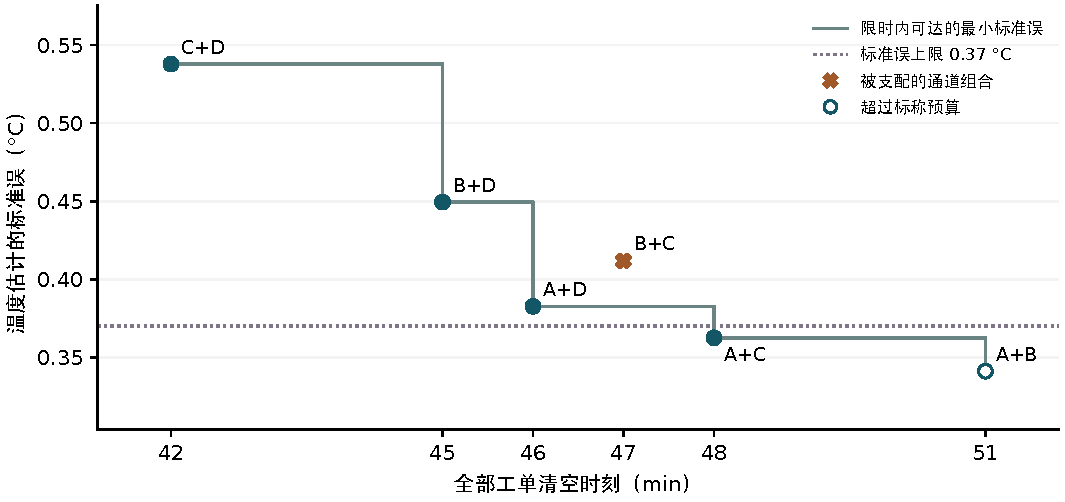
\includegraphics[width=.88\linewidth,height=.30\textheight,keepaspectratio]{joint_frontier.pdf}
\caption{测温标准误与全部五张工单最早清空时刻的关系。可选方案为离散的通道组合。}
\end{figure}
对六个通道组合分别评估全部 120 种工单顺序。对每个组合，B--C--D--A--E 都达到清空时刻下界 \(36+h_i+h_j\)，重新排列工单也无法消除新增的工位占用时间。在施加 12 仪器分钟的预算约束前，共有五个非支配组合。A+D 在两项指标上都优于 B+C：清空时刻从第 47 分钟提前至第 46 分钟，标准误从 \(0.412\) 降至 \(0.383^\circ\mathrm C\)。

在 12 仪器分钟预算内，要求第 46 分钟前（含该时刻）清空时应选 A+D；期限放宽至第 48 分钟，便可选 A+C，将标准误降至 \(0.362^\circ\mathrm C\)。若车间要求标准误不超过 \(0.37^\circ\mathrm C\)，最早可行的清空期限为第 48 分钟。额外耗时取决于通道准备是否实际占用检测工位，记录准备期间的工位占用情况即可判断应采用哪一版模型。
